%
% ait.tex
%
% Copyright (C) 2021 by SpaceLab.
%
% FloripaSat-2 Documentation
%
% This work is licensed under the Creative Commons Attribution-ShareAlike 4.0
% International License. To view a copy of this license,
% visit http://creativecommons.org/licenses/by-sa/4.0/.
%

%
% \brief AIT campaign.
%
% \author Gabriel Mariano Marcelino <gabriel.mm8@gmail.com>
%
% \institution Universidade Federal de Santa Catarina (UFSC)
%
% \version 0.1.0
%
% \date 2021/03/02
%

\chapter{Assembly, Integration and Test} \label{ch:ait}

AIT\nomenclature{\textbf{AIT}}{\textit{Assembly, Integration and Test.}}...

\section{Assembly Instructions}

\subsection{Preparation and Required Material}

\begin{itemize}
    \item .
    \item .
\end{itemize}

\subsection{Assembly Steps}

\begin{enumerate}
    \item .
    \item .
\end{enumerate}

\section{Environmental Testing}

\begin{itemize}
    \item Mass verification
    \item Dimensions verification (fit check)
    \item Center of gravity (CG\nomenclature{\textbf{CG}}{\textit{Center of Gravity.}}) verification
    \item Vibration test
    \item Thermal test
    \item Bake out test
\end{itemize}

\subsection{Mass, Center of Gravity and Fit Check}

\subsubsection{Mass Verification}

This test checks the total mass of the satellite (without RBF tag), which must be less than 2,66 kg \cite{cds}. The verification is made with a precision balance. \autoref{fig:mass-verification} examplifies this process with FloripaSat-I total mass.

\begin{figure}[!ht]
    \begin{center}
        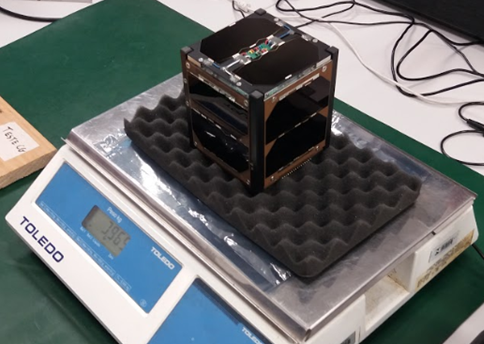
\includegraphics[width=0.5\textwidth]{figures/mass-test}
        \caption{Mass verificatiton of FloripaSat-I.}
        \label{fig:mass-verification}
    \end{center}
\end{figure}

\subsubsection{Center of Gravity}

This test checks the center of gravity (CG) of the satellite, which must be less than 2 cm from the geometric center (see \autoref{fig:cg}) \cite{cds}. To perform this test, a simple test-bench based on two parallel bars fixed on a plate (4 cm from each other) can be used. The geometric center of the satellite is put in the middle of the bars and, if the satellite does not fall, the CG is within the radius of 2 cm. This strategy does not measure the location of CG, however, it does prove if the satellite follows the requirement.

\begin{figure}[!htb]
    \begin{center}
        \subfigure[$X$ axis.\label{fig:fsat-fm-x-axis}]{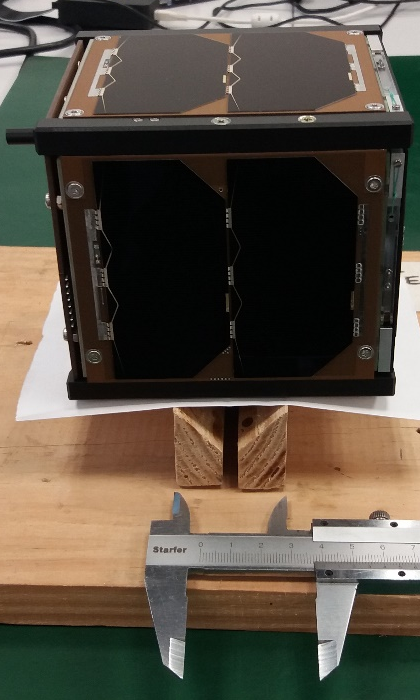
\includegraphics[width=0.2\textwidth]{figures/fsat_fm_x_axis.png}}
        ~
        \subfigure[$Y$ axis.\label{fig:fsat-fm-y-axis}]{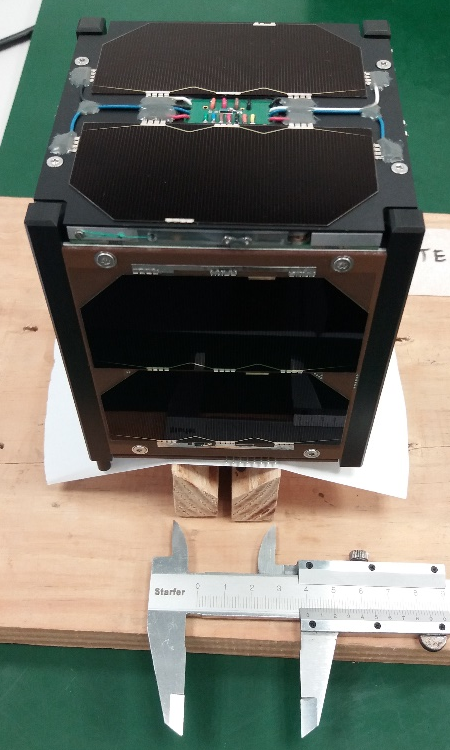
\includegraphics[width=0.2\textwidth]{figures/fsat_fm_y_axis.png}}
        ~
        \subfigure[$Z$ axis.\label{fig:fsat-fm-z-axis}]{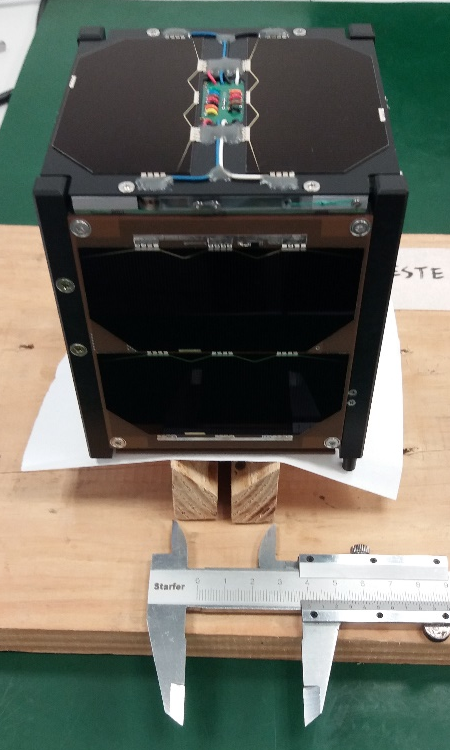
\includegraphics[width=0.2\textwidth]{figures/fsat_fm_z_axis.png}}
        \caption{Center of gravity of FloripaSat-I within 2 cm from geometric center.}
        \label{fig:cg}
    \end{center}
\end{figure}

\subsubsection{Fit Check}

\subsection{Vibration Test}

To measure and control the acceleration profile during the dynamic tests, accelerometers should be positioned on three external surfaces of the satellite, one on each axis, over areas without solar cells. The satellite should be fixed on a shaker. Figure \ref{fig:fsat-vibration-accel} shows some of the accelerometers and Figure \ref{fig:fsat-shaker} shows the satellite during a vibration test.

\begin{figure}[!htb]
    \begin{center}
        \subfigure[Position of the accelerometers.\label{fig:fsat-vibration-accel}]{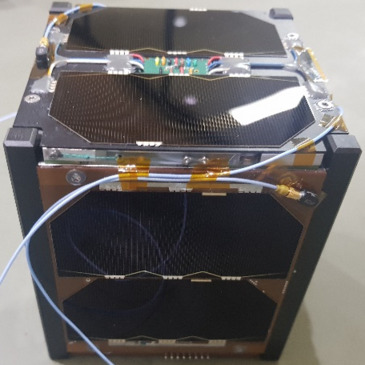
\includegraphics[height=4.5cm]{figures/fsat_fm_accel.jpg}}
        ~
        \subfigure[Shaker.\label{fig:fsat-shaker}]{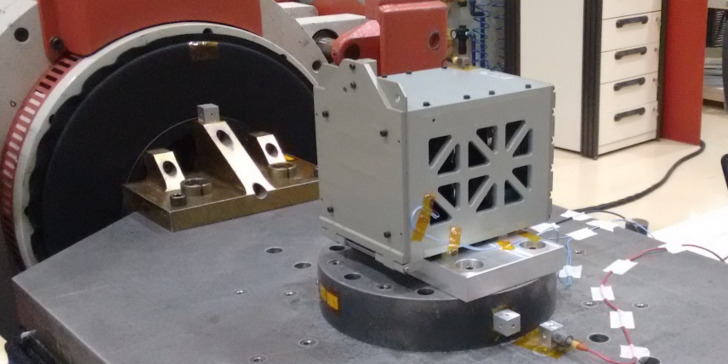
\includegraphics[height=4.5cm]{figures/fsat_fm_shaker.jpg}}
        \caption{Vibration test.}
        \label{fig:vibration-test}
    \end{center}
\end{figure}

The CubeSat should be tested entirely off, with RBF pin removed but with the Kill-Switches pressed, in a 2U Test POD, simulating the normal launching condition. The set of vibration tests follows \autoref{fig:vibration_procedure}.

\begin{figure}[!ht]
    \begin{center}
        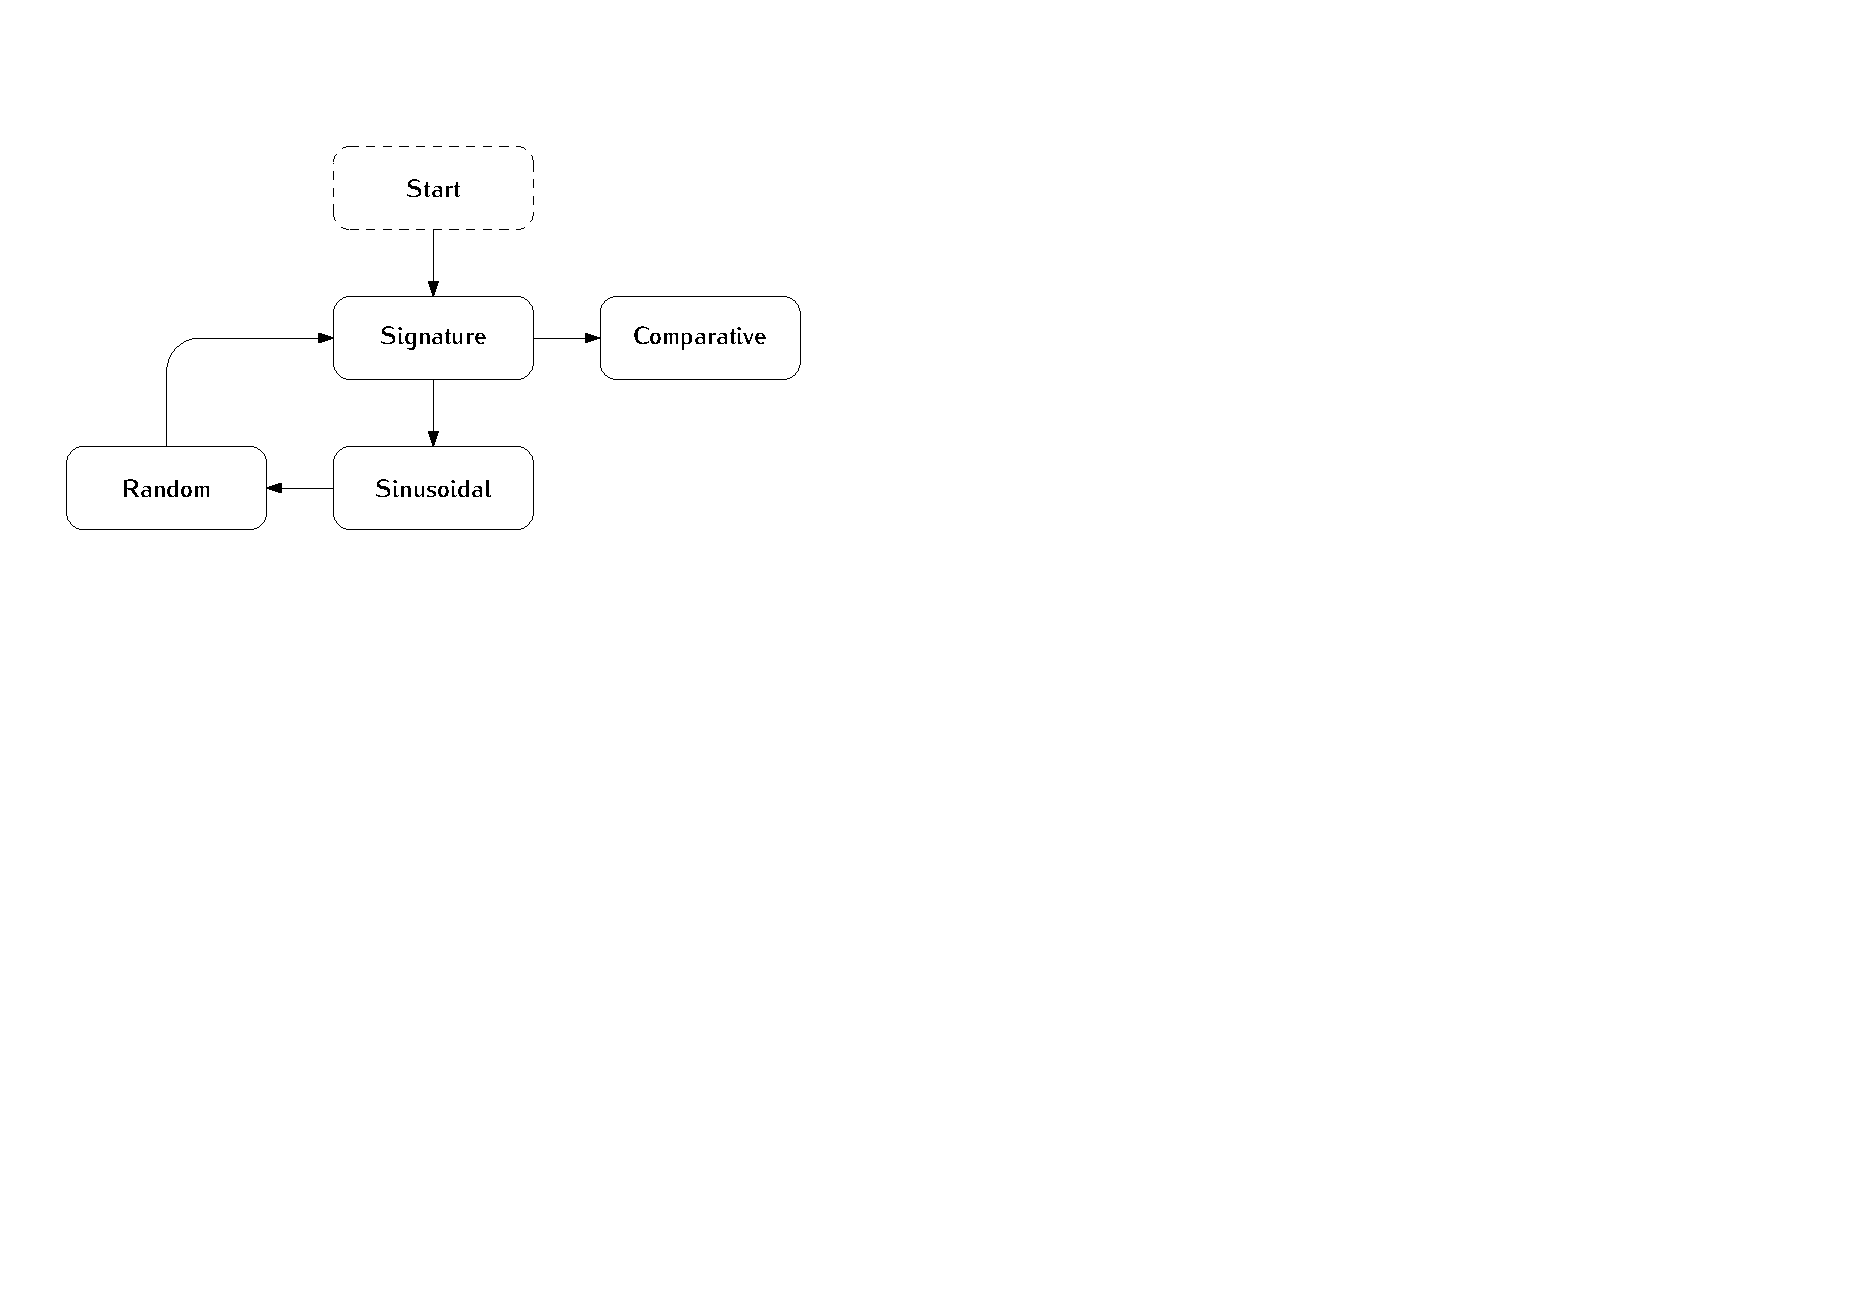
\includegraphics[width=0.6\textwidth]{figures/vibration_procedure.pdf}
        \caption{Sequence of dynamic tests.}
        \label{fig:vibration_procedure}
    \end{center}
\end{figure}

A signature testing should be conducted before and after the tests (sinusoidal and random vibration), in order to identify the presence of significant variations in the dynamic response, a condition that may represent mechanical failures. For the signature task, \autoref{tab:vibration-test-dynamic-1} presents the specifications.

\begin{table}[!h]
    \begin{center}
        \begin{tabular}{ll}
            \toprule[1.5pt]
            \textbf{Name}    & \textbf{Parameter}       \\
            \midrule
            Test method      & Sinusoidal sweep testing \\
            Frequency range  & 5 - 2000 Hz              \\
            Vibration level  & 0,25 g                   \\
            Sweep rate       & 2 octaves per minute     \\
            Number of sweeps & 1 (5 - 2000 Hz)          \\
            Test axes        & 3 ($X$, $Y$, $Z$)        \\
            \bottomrule[1.5pt]
        \end{tabular}
        \caption{Resonance survey test (signature).}
        \label{tab:vibration-test-dynamic-1}
    \end{center}
\end{table}

%Regarding the sinusoidal sweeping vibration, Table 3 brings the envelope of the test, and so does Fig. 24 in a graphic format.

\begin{figure}[!ht]
    \begin{center}
        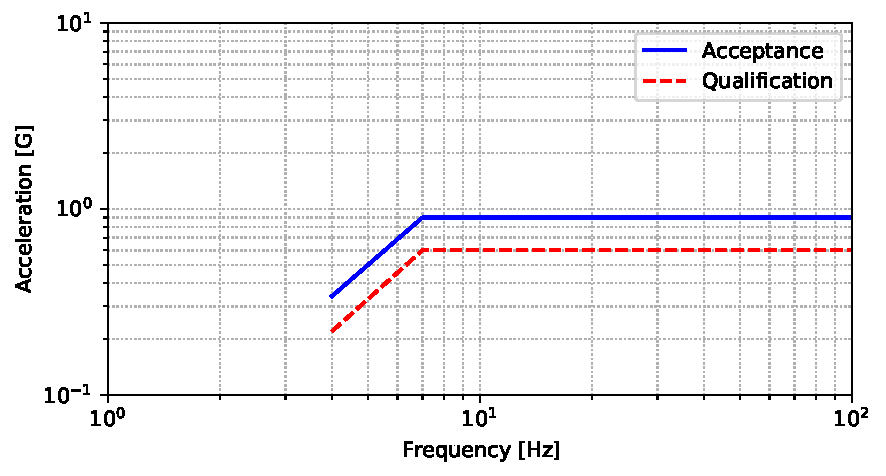
\includegraphics[width=\textwidth]{curves/sine_test.pdf}
        \caption{Sinusoidal sweeping vibration curve.}
        \label{fig:vibration-sinusoidal-curve}
    \end{center}
\end{figure}

\begin{figure}[!ht]
    \begin{center}
        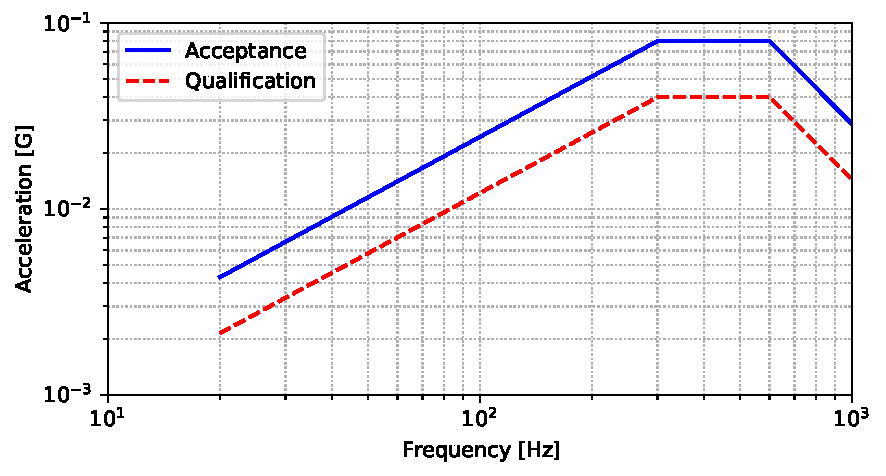
\includegraphics[width=\textwidth]{curves/random_vibration.pdf}
        \caption{Random vibration curve.}
        \label{fig:vibration-test}
    \end{center}
\end{figure}

\subsection{Thermal Cycling}

For the thermal tests, thermocouples should be attached on different points on the surface of the satellite, including over the solar panels and structure. As an example, \autoref{fsat-thermal-test} shows FloripaSat-I ready for thermal tests. The parameters of the tests are indicated in \autoref{tab:fsat-thermal-cycling}.

\begin{figure}[!ht]
    \begin{center}
        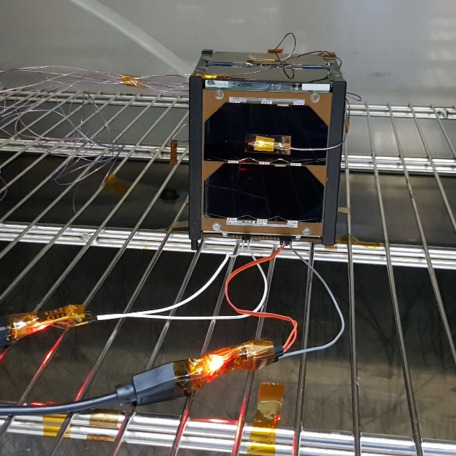
\includegraphics[width=0.5\textwidth]{figures/fsat_fm_thermal_cycling.jpg}
        \caption{FloripaSat-I during the thermal cycling (with thermocouples).}
        \label{fig:fsat-thermal-test}
    \end{center}
\end{figure}

\begin{table}[!h]
    \begin{center}
        \begin{tabular}{llll}
            \toprule[1.5pt]
            \multicolumn{2}{c}{\textbf{Thermal cycle}}  & \multicolumn{2}{c}{\textbf{Bake out}}        \\
            \midrule
            \textbf{Parameter}     & \textbf{Value}     & \textbf{Parameter} & \textbf{Value}          \\
            \midrule
            Number of cycles       & 2                  & \multicolumn{2}{c}{Part 1}                   \\
            \cmidrule{3-4}
            Min. temp. ($T_{min}$) & -15 $^\circ$C      & Pressure           & <1$\times 10^{-4}$ mbar \\
            Max. temp. ($T_{max}$) & +50 $^\circ$C      & Temperature        & 23 $^\circ$C            \\
            Duration in $T_{min}$  & 30 min             & Duration           & 12 hours                \\
            \cmidrule{3-4}
            Duration in $T_{max}$  & 60 min             & \multicolumn{2}{c}{Part 2}                   \\
            \cmidrule{3-4}
            Heating rate           & 5.5 $^\circ$C/min  & Pressure           & <1$\times 10^{-4}$ mbar \\
            Cooling rate           & 3.5 $^\circ$C/min  & Temperature        & 60 $^\circ$C            \\
            Stabilization criteria & 1 $^\circ$C/10 min & Duration           & 6 hours                 \\
            \bottomrule[1.5pt]
        \end{tabular}
        \caption{Parameters for the bake out and thermal cycling.}
        \label{tab:fsat-thermal-cycling}
    \end{center}
\end{table}

\subsection{Bake Out}

\begin{enumerate}
    \item .
    \item .
\end{enumerate}

\section{Pre-launch Preparation}

\begin{enumerate}
    \item .
    \item .
\end{enumerate}

\subsection{Keys of the Telecommands}

\begin{enumerate}
    \item .
    \item .
\end{enumerate}

\subsection{Firmware Upload}

\begin{enumerate}
    \item .
    \item .
\end{enumerate}

\subsection{Memory Reset}

\begin{enumerate}
    \item .
    \item .
\end{enumerate}

\section{Transport to Launch}

\subsection{Packing the Satellite}

\begin{enumerate}
    \item .
    \item .
\end{enumerate}

\subsection{Unpacking the Satellite}

\begin{enumerate}
    \item .
    \item .
\end{enumerate}
